\documentclass[a4paper,oneside,DIV=12,12pt]{scrartcl}

\usepackage{graphicx}

\usepackage{fontspec}
\setmainfont{PT Serif}
\setsansfont{PT Sans}
\setmonofont{PT Mono}

\usepackage{unicode-math}
\setmathfont{PT Serif}

\usepackage{microtype}

\usepackage{polyglossia}
\setmainlanguage{ukrainian}
\setotherlanguage{english}

\usepackage{xcolor}

\usepackage{hyperref}
\hypersetup{
	colorlinks      = false,%
	linkbordercolor = blue,%
	pdfborderstyle  = {/S/U/W 1},%
}

%%% Itemize and enumerate customization
\usepackage{enumitem,calc}
\setlist[itemize]{label=—}
%%%

%%%
\usepackage{listings}
\usepackage{lstautogobble}
\lstset{
	basicstyle = \ttfamily,
	breaklines = true,
	columns    = fullflexible,
	autogobble,
}
%%%

%%% Table typesetting
% \usepackage{array}
% \newcolumntype{v}[1]{>{\raggedright\arraybackslash\hspace{0pt}}p{#1}}
% \newcolumntype{n}[1]{>{\raggedleft\arraybackslash\hspace{0pt}}p{#1}}
%%%

%%% Count figures within issues (sections)
\usepackage{chngcntr}
\counterwithin{figure}{section}
%%%

\newcommand{\progname}{tinyplot}

\newcommand{\theprojcode}{PLOTSCRIPT}
\newcommand{\theprojrev}{00}
\newcommand{\thedoctype}{BUGREPORTS}
\newcommand{\thedocnum}{000}
\newcommand{\thedocfullcode}{\theprojcode-\theprojrev-\thedoctype-\thedocnum}
\newcommand{\printdocfullcode}{\texttt{\thedocfullcode}}
\newcommand{\theversion}{2017-12-07-000}

\newcommand{\classname}[1]{\texttt{#1}}
\newcommand{\funcname}[1]{\texttt{#1}}

\newcommand{\bugattrib}[1]{\noindent\textbf{#1}}

\newcommand{\printtrue}{\texttt{True}}
\newcommand{\printfalse}{\texttt{False}}

\newcommand{\filename}[1]{\texttt{#1}}

%%% Create new Steps environment
\DeclareDocumentEnvironment{steps}%
{O{}}% If no argument is given the label defaults to 'Step'
{\begin{enumerate}[leftmargin = *]}% Tune labelindent to set hanging step number
{\end{enumerate}}
%%%

\setcounter{tocdepth}{1}

\begin{document}
	\begin{titlepage}
	\begin{center}
		\vspace*{\fill}
			Звіт про дефекти\\
			виявлені під час тестування\\
			програмного продукту для побудови графіків
			
		\vspace*{\fill}
	\end{center}
	Кодова назва проекту: \theprojcode\\
	Код документу: \printdocfullcode\\
	Версія: \theversion\\
	\end{titlepage}
	
	\tableofcontents
	\newpage
	
	\section{Помилка \texttt{FileNotFoundError}}
		\subsection{Ідентифікатор}
			5.
			
		\subsection{Повідомила}
			Ульчич Ірина.
			
		\subsection{Короткий опис}
			Помилка \verb|FileNotFoundError| під час спроби відкрити файл.
			
		\subsection{Кроки для відтворення}
			\begin{steps}
				\item Запустити програму для обробки неіснуючого файлу.
					\begin{lstlisting}
						tinyplot\tinyplot.py nonexistent-file
					\end{lstlisting}
					
				\item Спостерігати результат.
			\end{steps}
			
		\subsection{Яка поточна некоректна поведінка?}
			Під час спроби обробити неіснуючий файл помилка \verb|FileNotFoundError| не оброблюється.
			
		\subsection{Яка очікується коректна поведінка?}
			Під час спроби обробити неіснуючий файл помилка \verb|FileNotFoundError| коректно оброблюється та попереджає користувача, радячи перевірити назву файлу при наступному запуску.
			
		\subsection{Логи і скріншоти}
			Вивід командного рядка наведений нижче.
			\begin{lstlisting}
Traceback (most recent call last):
  File "tinyplot\tinyplot.py", line 188, in <module>
    main(args)
  File "tinyplot\tinyplot.py", line 106, in main
    raw_coordinates = get_raw_coordinates(args.input)
  File "tinyplot\tinyplot.py", line 52, in get_raw_coordinates
    with open(f, 'r') as infile:
FileNotFoundError: [Errno 2] No such file or directory: 'asdf'
			\end{lstlisting}
			
			Версії встановлених програм:
			\begin{lstlisting}
				$ python --version
				Python 3.6.3

				$ pip3 list
				cycler (0.10.0)
				matplotlib (2.1.0)
				numpy (1.13.3)
				pip (9.0.1)
				pyparsing (2.2.0)
				python-dateutil (2.6.1)
				pytz (2017.3)
				setuptools (38.2.4)
				six (1.11.0)
				tinyplot (0.1.0.dev0)
			\end{lstlisting}
			
		\subsection{Можливі способи виправлення}
			Оточити ділянку коду, що відповідає за відкриття файлів конструкцією такого вигляду:
			\begin{lstlisting}
				try:
					...
				except:
					...
			\end{lstlisting}
			
			У разі виявлення помилки попередити користувача.
			
	\section{Відсутня обробка нульової ціни поділки}
		\subsection{Ідентифікатор}
			6.
		
		\subsection{Повідомив}
			Рабін Ігор.
			
		\subsection{Короткий опис}
			Помилка \verb|ValueError: Maximum allowed size exceeded|.
			
		\subsection{Кроки для відтворення}
			\begin{steps}
				\item Запустити програму, встановивши для параметра \texttt{xtickvalue} значення 0.
				\begin{lstlisting}
				> tinyplot.py test --xtickvalue 0
				\end{lstlisting}
				
				\item Спостерігати результат.
			\end{steps}
			
		\subsection{Яка поточна некоректна поведінка?}
			Якщо встановити нульове значення ціни поділки, то програма не здатна побудувати графік і ніяк не оброблює цей граничний випадок~— завершує роботу з помилкою.
		\subsection{Яка очікується коректна поведінка?}
			Програма повинна обробити значення, попередити користувача, що неможливо побудувати графік з нульовою ціною поділки. Можливо, навіть встановити певне \emph{fall-back} значення.
			
		\subsection{Логи і скріншоти}
			\begin{lstlisting}
				tinyplot\tinyplot.py:144: RuntimeWarning: divide by zero encountere
				d in double_scalars
				  plt.xticks(np.arange(start, end, args.xtickvalue))
				Traceback (most recent call last):
				  File "tinyplot\tinyplot.py", line 188, in <module>
					main(args)
				  File "tinyplot\tinyplot.py", line 144, in main
					plt.xticks(np.arange(start, end, args.xtickvalue))
				ValueError: Maximum allowed size exceeded
			\end{lstlisting}

			Версії встановлених програм:
			\begin{lstlisting}
				$ python --version
				Python 3.6.2

				$ pip3 list
				cycler (0.10.0)
				matplotlib (2.1.0)
				numpy (1.13.3)
				pip (9.0.1)
				pyparsing (2.2.0)
				python-dateutil (2.6.1)
				pytz (2017.3)
				setuptools (38.2.4)
				six (1.11.0)
				tinyplot (0.1.0.dev0)
			\end{lstlisting}
			
	\section{Відсутність повідомлення про нестачу даних}
		\subsection{Ідентифікатор}
			7.
			
		\subsection{Повідомив}
			Моложанов Леон.
			
		\subsection{Короткий опис}
			Якщо програмі не вдалось зчитати достатню кількість даних для побудови графіка, вона не попереджує про це.
			
		\subsection{Кроки для відтворення}
			\begin{steps}
				\item Пересвідчитись, що у вхідному файлі відсутні коректні дані (для цього видалити його зміст, ввести некоректні дані тощо).
				\item Запустити програму для обробки вищезгаданого вхідного файлу.
				\item Спостерігати результат.
			\end{steps}
			
		\subsection{Яка поточна некоректна поведінка?}
			Програма будує пустий графік, не попереджуючи користувача.
			
		\subsection{Яка очікувана коректна поведінка?}
			Програма попереджує користувача про нестачу даних та завершує роботу.
			
		\subsection{Логи і скріншоти}
			Версії встановлених програм:
			\begin{lstlisting}
				$ python --version
				Python 3.6.2

				$ pip3 list
				cycler (0.10.0)
				matplotlib (2.1.0)
				numpy (1.13.3)
				pip (9.0.1)
				pyparsing (2.2.0)
				python-dateutil (2.6.1)
				pytz (2017.3)
				setuptools (38.2.4)
				six (1.11.0)
				tinyplot (0.1.0.dev0)
			\end{lstlisting}
			
			Результат неправильної роботи програми зображений на рис.~\ref{fig:issue-007-01}.
			
			\begin{figure}[!htbp]
			\centering
				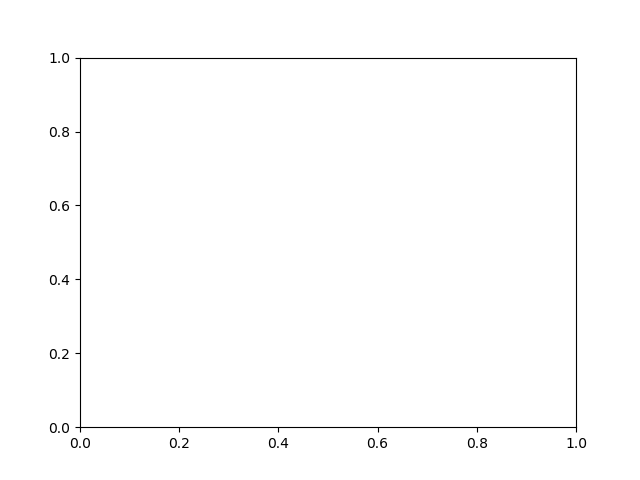
\includegraphics[height = 9\baselineskip]{assets/issue-007-01.png}
			\caption{Результат неправильної роботи програми}
			\label{fig:issue-007-01}
			\end{figure}
			
	\section{Відсутність деталей при ігноруванні некоректних даних}
		\subsection{Ідентифікатор}
			8.
			
		\subsection{Повідомив}
			Нагнибіда Олександр.
			
		\subsection{Короткий опис}
			Якщо вхідний файл містить некоректні дані, програма ігнорує їх, не попереджуючи користувача незалежно від налаштувань.
			
		\subsection{Кроки для відтворення}
			\begin{steps}
				\item Ввести у вхідний файл некоректні дані. Наприклад:
					\begin{lstlisting}
						1.0-1 2.2*2
						3.3^3 4.8/2
					\end{lstlisting}
					
				\item Запустити програму для роботи над вхідним файлом.
					\begin{lstlisting}
						tinyplot.py incorrect_data.txt
					\end{lstlisting}
				
				\item Спостерігати результат.
			\end{steps}
			
		\subsection{Яка поточна некоректна поведінка?}
			Програма не повідомляє про ігнорування рядків з некоректними даними, які не враховуються при побудові графіка.
			
		\subsection{Яка очікується коректна поведінка?}
			Програма повідомляє користувача про конкретні рядки, які були проігноровані під час побудови графіка.
			
		\subsection{Логи і скріншоти}
			Версії встановлених програм:
			\begin{lstlisting}
				$ python --version
				Python 3.6.2

				$ pip3 list
				cycler (0.10.0)
				matplotlib (2.1.0)
				numpy (1.13.3)
				pip (9.0.1)
				pyparsing (2.2.0)
				python-dateutil (2.6.1)
				pytz (2017.3)
				setuptools (38.2.4)
				six (1.11.0)
				tinyplot (0.1.0.dev0)
			\end{lstlisting}
			
		\subsection{Можливі способи виправлення}
			Можна ввести флаг \verb|--verbose| для більшої деталізації процесу роботи.
\end{document}
